\section{Grader} \label{sec:grader}
Når man arbejder med grafer, kan det være brugbart at vide, hvor mange kanter der er incidente med en knude. Dertil bruger man følgende definition:

\begin{defn}[Grader] \label{defn:grader}
Lad $v \in V$ være en knude i den simple ikke-orienterede graf, $G = (V,E)$. Knudens antal \emph{grader}, $\deg(v)$, er det antal kanter i $E$, som er incidente med $v$. Dermed gælder det, at
\begin{equation}
\deg(v)=|\{u \in V: \{u,v\} \in E \}|,
\end{equation}
\end{defn}

Hvis der ikke er tale om en simpel graf, men derimod en pseudograf, skal man være opmærsom på de multiple kanter og løkker, når man tæller antallet af knudens grader. Hvis der er multiple kanter, tælles alle disse med, og løkker tæller dobbelt, idet de både starter og slutter i knuden.

\begin{exmp} \label{ex:grader}

Vi kan ud fra dette aflæse knudernes grader på \autoref{fig:grader}, $\deg(v_{1})=3, \ \deg(v_{2})=3, \ \deg(v_{3})=4$ og $\deg(v_{4})=4$. En knudes grader afgøres altså af, hvor mange kanter, der er incident med knuden, medmindre knuden har en løkke, da man her kun siger, at kanten kun er incident med knuden én gang, men den tæller dobbelt i antallet af grader.


\begin{figure}[H]
\centering
	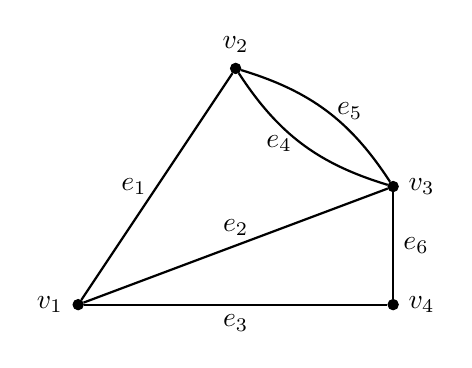
\begin{tikzpicture}[every loop/.style={}]
      \tikzset{enclosed/.style={draw, circle, inner sep=0pt, minimum size=.13cm, fill=black}}
%% Vertices
      	\node[enclosed, label={left: $v_1$}] (v1) at (0,0) {};
      	\node[enclosed, label={above: $v_2$}] (v2) at (2,3) {};
    	\node[enclosed, label={right: $v_3$}] (v3) at (4,1.5) {};
  	    \node[enclosed, label={right: $v_4$}] (v4) at (4,0) {};
%Edges
		\path[thick] (v2) edge [bend right=20] node[midway, left] {$e_4$} (v3);
		\path[thick] (v3) edge [bend right=20] node[midway, right] {$e_5$} (v2);
		\path[thick] (v1) edge node[midway, above] {$e_2$} (v3);
		\path[thick] (v1) edge node[midway, below] {$e_3$} (v4);
		\path[thick] (v1) edge node[midway, left] {$e_1$} (v2);
		\path[thick] (v3) edge node[midway, right] {$e_6$} (v4);
	\end{tikzpicture}
	\caption{Multigraf.}
	\label{fig:grader}
\end{figure}


\end{exmp}

\begin{thm}
Lad grafen, $G = (V,E)$, være en ikke-orienteret graf med E antal kanter. Knuden $v$ har $deg(v)$ antal grader, og det gør sig derfor gældende, at
\begin{equation}
	\sum_{v \in V} { } \deg(v) = 2 \cdot |E|.
\end{equation}
Dette gælder, så længe grafen ikke er uendelig.
\end{thm}
Hvis vi har en ikke-orienteret, endelig graf, kan man altså finde antallet af kanter i grafen ved at lægge summen af hver knudes grader sammen og dividere dette tal med to.

\begin{proof}
Som det fremgår af Definition \ref{def:graf}, er multimængden af kanter, $E \subseteq \{\{u,v\}|u,v \in V \}$. Hver kant i grafen er altså incident med to punkter, eller med det samme punkt to gange, hvis der er tale om en løkke. Hvis en kant er incident med en knude, bidrager denne kant til knudens grader, $\deg{v}$. Hver kant bidrager altså to gange til det samlede antal grader. Derfor vil hele grafens antal grader, $\sum_{v \in V} { } \deg(v)$, være dobbelt så stor, som antallet af kanter i denne graf, $|E|$. Derfor får vi at 
\begin{equation}
2 \cdot |E|= \sum_{v \in V} { } \deg(v).
\end{equation} 
\end{proof}

I en orienteret graf tælles knudernes grader på anden vis. I en orienteret graf er en knude, $u$, incident med en anden knude $v$, hvis en orienteret kant har $u$ som sit startpunkt og $v$ som sit endepunkt. Derfor tælles antallet af grader i en orienteret graf i \emph{indadgående} grader og \emph{udadgående} grader. 
For knuden $v$ betegner $\deg^{-}(v)$ antallet af de indadgående kanter, altså de kanter, der har $v$, som sit endepunkt. Modsat betegner $\deg^{+}(v)$ antallet af de udadgående kanter, altså de kanter, der har $v$, som sit startpunkt. Da hver kant skal have både et start og et endepunkt, må det gælde at:
\begin{equation}
|E|=\sum_{v \in V} { } \deg^{-}(v) = \sum_{v \in V} { } \deg^{+}(v).
\end{equation}

\begin{exmp} \label{ex:grader_orienteret}
Vi kan nu beregne antallet af indadgående og udadgående grader i \autoref{fig:grader_orienteret}.
\input{fig/tikz/grafer/grader_orienteret_eksempel}
Vi ser, at $\deg^{+}(v_{1})=3$, $\deg^{-}(v_{1})=0$, $\deg^{+}(v_{2})=1$, $\deg^{-}(v_{2})=2$, $\deg^{+}(v_{3})=2$, $\deg^{-}(v_{3})=2$, $\deg^{+}(v_{4})=1$ og $\deg^{-}(v_{4})=3$. Vi ser altså, at en løkke tæller som både en indadgående kant og en udadgående kant.
\end{exmp}